\section{Dynamic Programming} \index{dynamic programming} \index{memoization}

\textit{\textbf{Dynamic programming}} (DP) is a method for solving complex problem by breaking it down to a collection of simpler subproblems, solving each of those subproblems, and storing their solutions. The next time the same subproblem occurs, instead of recomputing the solution, the algorithm can just use the previously computed solution. Each subproblem is indexed in some way to facilitate the lookup. The technique of storing solutions to subproblems is called \textbf{memoization}.

Let's consider the weighted interval selection problem.

\section{Weighted Interval Selection}

The objective of the weighted interval selection problem is to find a non-intersecting set of intervals so that the sum of the weights of intervals in the set is minimized. More formally, given a set of jobs/activities $\{a_1,\ldots,a_n\}$ with start time $s_i$ and finish time $f_i$ and weight $w_i$, we want to find a set $S$ of mutually compatible jobs with highest total weight $\sum_{i \in S} w_i$ 

Note that when $w_i = 1$ for all $i = \{1,\ldots,n\}$, the weighted interval selection problem is the same as simple interval scheduling.

We first consider greedy algorithms. Possible choices for the greedy choice include: weights, interval length, etc. Unfortunately, all the possible ways of ordering the input items will not only fail to give an optimal solution, but can in fact produce arbitrarily bad solutions for some instances. With a generalized greedy approach, it can be proved that no greedy algorithm can produce a good solution. With certain modifications/extensions to greedy, the algorithm can produce a good approximation (by allowing revocable decisions) and even optimal solution (using local ratio/primal dual algorithms with a reverse delete phase).

\section{Computing the Optimal Weight}
\subsection{The Dynamic Programming Approach}

Assume that the jobs (intervals) have been sorted by non-decreasing finish time. Then, in an optimal solution $O$, either the last interval $I_n$ was selected, or it was not. If not, then we must be using an optimal solution for the first $n-1$ intervals. If $a_n$ is in $O$, then no interval in $O$ can end after the starting time of $a_n$.

Let us now make this intuition more concrete. Given that the jobs are sorted by non-decreasing finish time, let $\id{pred}(i)$ be the largest index $j < i$ such that $f_j < s_j$. This means that jobs $a_1,\ldots,a_j$ are compatible with $a_i$, but $a_{i+1},\ldots,a_{j-1}$ are not compatible.

Let $O$ be an optimal solution. For each job $a_i$, there are two possibilities:
\begin{itemize}
    \item Job $a_i \in O$: This implies that $\{\id{pred}[i]+1,\ldots,a_{i-1}\}$ are all incompatible with $a_i$. So, we must select jobs from $\{a_1,\ldots,\id{pred}[i]\}$.
    
    \begin{center}
        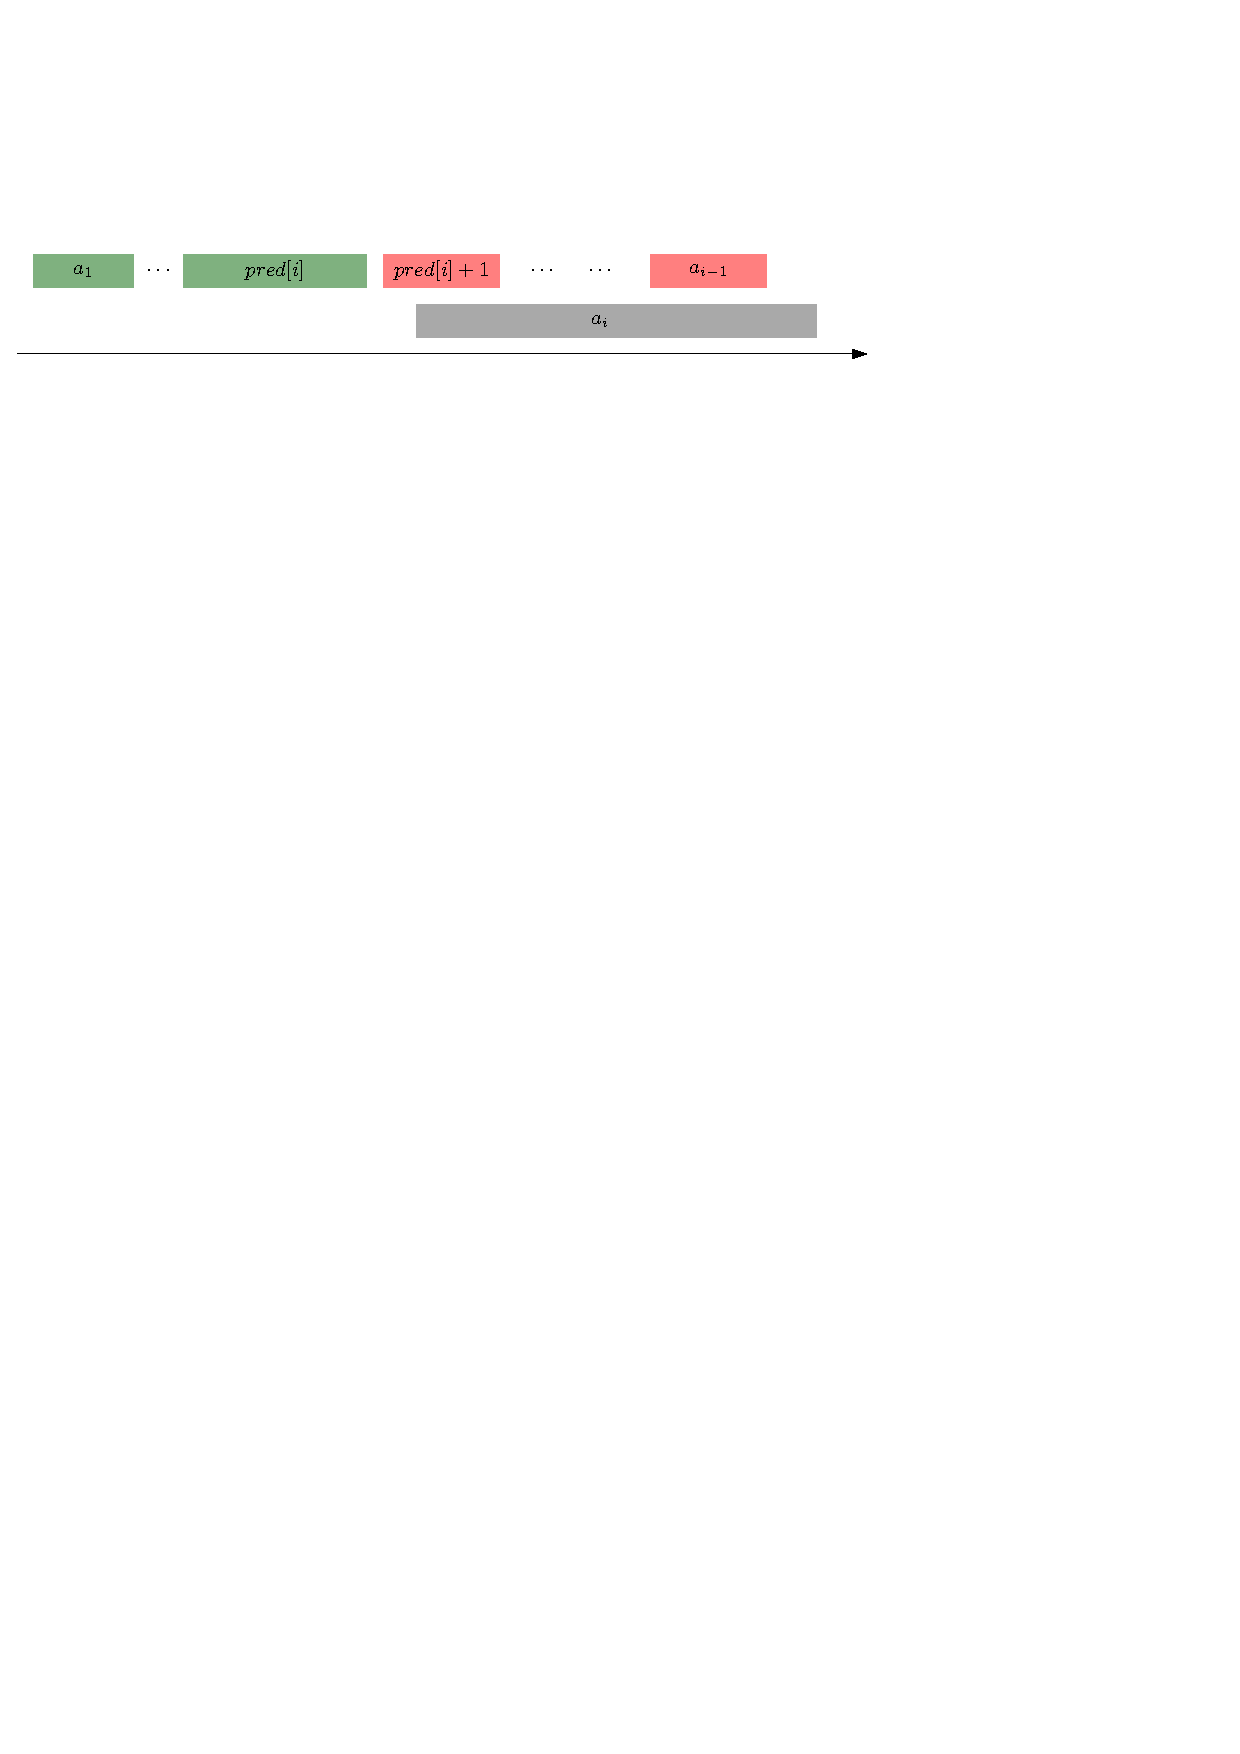
\includegraphics[width=0.8\linewidth]{dp/wisp/wisp-opt-case1.pdf}
    \end{center}

    \item Job $a_i \not\in O$: This implies that we must select jobs from $\{a_1,\ldots,a_{i-1}\}$. 
    
    \begin{center}
        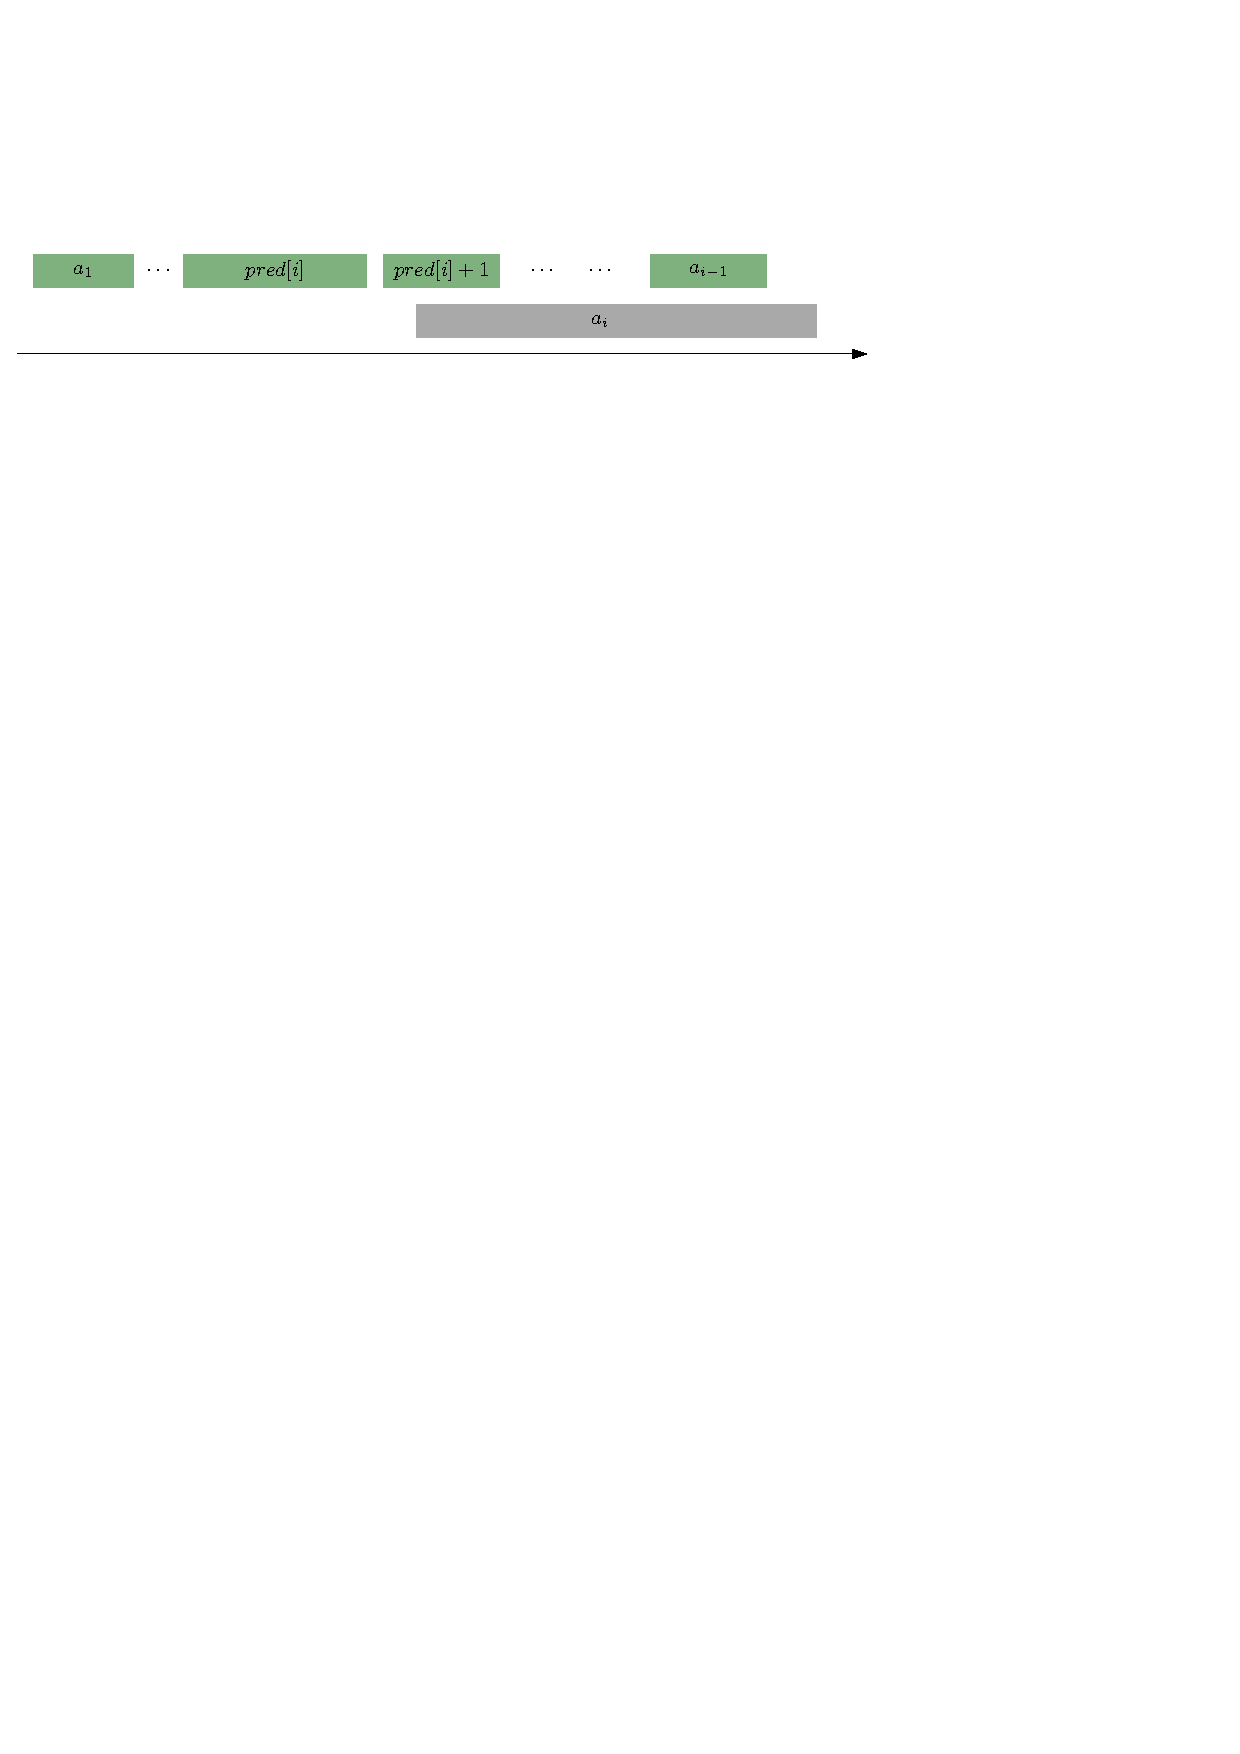
\includegraphics[width=0.8\linewidth]{dp/wisp/wisp-opt-case2.pdf}
    \end{center}
\end{itemize}

Let define $V:\; \{a_1,\ldots,a_n\} \to \R$ be defined such that
$$
V(i) = \text{max total weight of compatible jobs from $\{a_1,\ldots,a_i\}$}
$$
More formally, $V$ can be expressed as this recurrence
$$
V(i) = \begin{cases}
    0 & i = 0 \\
    \max \{V(i-1),w_i+V(\id{pred}[i]) \} & i > 0
\end{cases}
$$
\begin{lemma}
    The two definitions of $V$ are equivalent.
\end{lemma}
\begin{proof}
    By induction.
\end{proof}
\index{semantic array} \index{Bellman equation}
Sometimes, the first definition of $V$ in English is represented as an array indexed by $i$ and referred to as a \textit{\textbf{semantic array}}. The second equation of $V$ is called the \textit{\textbf{Bellman equation}}.

This recurrence gives us a clear recursive solution for the weighted interval selection problem.

Consider the time complexity of the naive recursive implementation. $\id{pred}[i]$ can be computed using binary search in $O(\log n)$ time, and for all of the $n$ values to be considered, this takes $O(n \log n)$ time. However, the time spent on computing $\id{pred}$ turns out to be rather insignificant compared to the running time of the main algorithm.
$$
T(n) = T(n-1) + T(\id{pred}[n]) \leq T(n-1) + T(n-2) \in \Theta(\varphi^n)
$$
where $\varphi \approx 1.618$ is the golden ratio. This is a Fibonacci recurrence.

This is clearly bad. Some solutions are being computed many times unnecessarily. Recall that one of the most important component of dynamic programming is memoization. In many cases, without memoization, dynamic programming simply becomes divide and conquer, or even worse, recurrence that runs in exponential time like this one. Memoization allows us to remember the results that we have already computed and reuse them if needed.

\subsection{Top-Down DP}
In our first dynamic programming implementation, we will store the previously computed values in the array $M$ indexed by the index of each interval.

Assume that prior to calling $\proc{Compute-Opt-DP}(n)$, the intervals are sorted in nondecreasing order based on finish time, $\id{pred}$ has been precomputed in $O(n\log n)$ time, and $M$ is a global array of size $n$ with every entry set to 0 initially.

\begin{codebox}
    \Procname{$\proc{Compute-Opt-DP}(j)$}
    \li \If $M[j] \isequal \const{nil}$ \Then 
        \li $M[j] = \max\{\proc{Compute-Opt-DP}(j-1),\; w_j + \proc{Compute-Opt-DP}(\index{pred}[j]) \}$
    \End
    \li \Return $M[j]$
\end{codebox}

For each $i = \{1,\ldots,n\}$, there is only one call to $\proc{Compute-Opt-DP}(i)$ because previously computed values are stored in the array $M$. Therefore, there are at most $O(n)$ calls to the recursive procedure. Sorting by finish time and computing $\id{pred}$ takes $O(n \log n)$ time, so the overall time complexity of this implementation is $O(n \log n)$. Much better than our original exponential implementation!

\subsection{Bottom-Up DP}

The bottom-up approach differs from the top-down approach in that values of $M$ are precomputed. Instead of using recursive call and checking if $M[i] \isequal \const{nil}$, we can simply reference to indices of the array where previously computed values are stored. Assume the same preconditions are met prior to calling \proc{Compute-Opt-DP-Botton-Up}.

\begin{codebox}
    \Procname{$\proc{Compute-Opt-DP-Botton-Up}()$}
    \li \For $j = 1$ to $n$ \Do
        \li $M[j] = \max\{M[j-1],\, w_j + M[\id{pred}[j]] \}$
    \End
    \li \Return $M[n]$ 
\end{codebox}

It can be shown using a simple loop invariant and induction that at the beginning of the $i$th iteration, $M[j]$ is already computed for all $j < i$ and thus we will not get a null pointer error.

This approach has the same time complexity as the top-down approach.

\subsection{Comparison of Two Approaches}

Top-down may be preferred when not all sub-solutions need to be computed on some inputs. This helps us save some time.

Bottom-up may be preferred when all sub-solutions will always need to be computed for all inputs. The bottom-up approach could be faster as it prevents unnecessary recursive calls which results in unnecessary random memory access. This is because even though recursive dynamic programming does not compute repeated results, there could still be redundant recursive calls, resulting in a large overhead.

\section{Computing the Optimal Solution}

In the previous section, we come up with a dynamic programming algorithm that computes the optimal weight of the solution set for the weighted interval selection problem. Now, we will extend that algorithm so that we get the actual solution set (subset of $S$ that maximizes weight). We only need a really simple modification from the original definition of $V$. Recall that $V$ is defined as
$$
V(i) = \begin{cases}
    0 & i = 0 \\
    \max \{V(i-1),w_i+V(\id{pred}[i]) \} & i > 0
\end{cases}
$$
Instead of calculating values, we want a subset of the input set.
$$
S(i) = \begin{cases}
    \emptyset & i = 0 \\
    S(i-1) & \text{if $V(i) = V(i-1)$} \\
    S(\id{pred[i]}) \cup \{ a_i \} & \text{otherwise}
\end{cases}
$$
We can either precompute $V$ and uses it directly in the implementation of $S$. Or alternatively, we can compute $V$ and $S$ simultaneously.